\documentclass[11pt]{article}

% Include useful packages
\usepackage{graphicx}
\usepackage{acl-hlt2011}
\graphicspath{ {images/} }
\usepackage{float}
\usepackage[utf8]{inputenc}
\usepackage{amsmath}
\usepackage{amsfonts}
\usepackage{amssymb}
\usepackage{arabtex}
\usepackage{CJKutf8}
\usepackage{times}
\usepackage{latexsym}
\usepackage{multirow}
\usepackage{url}
\DeclareMathOperator*{\argmax}{arg\,max}


\begin{document}

% Copyright
%\setcopyright{acmcopyright}


\title{Short Text Language Detection with Twitter}

\author{Jun Du \\
  {\tt dujun1@msu.edu} \\\And
  Ruochuan Zhang \\
  {\tt zhangr12@msu.edu} \\}

\date{}

\maketitle
\section{Abstract}
Identifying the language of a text is an important requirement
for any other processing on written text. While the
focus so far has been mainly on language detection for long
written text, short social media post like tweets are becoming
more important. Furthermore, most language classifiers
are designed to work only with dozens of languages. In this
final report, we scale up the language identification to work on
200 languages, and additionally present the results of the
classifier on a twitter data set of 79 languages. The classifier
reached close to 95\% when tested on 200 languages,
and the results on the twitter data set are just short of 90\%.


\section{Introduction}
Many automated language detectors exist, but most only
work on the order of dozens of languages and focus on European
languages. Meanwhile, hundreds of languages are
spoken around the world, and many of these, although we
never heard about them, are spoken by millions of people.
As more and more people around the world, especially in
Asia, but also Africa, begin to use social media websites like
Twitter and Facebook, these languages are becoming better
represented online. So, NLP technologies on these sites need
to be equipped to handle the main spoken languages of the
world, not just the most popular few.
We intend to build a language classifier for Twitter, training
on a corpus of approximately 200 languages. Specifically,
this classifier should be able to make a decision between
these languages when given only a single tweet as input.
Working with tweets will present some unique challenges.
Because tweets are only 140 characters long, at most, we
cannot gather statistics that require a large count of words.
Also, dealing with colloquial language and misspellings will
need to be considered.


\section{Dataset}
There are many translation text data corpora out there,
but few cover more than several dozen up to a hundred languages. The ones which do cover the number of languages
we need typically don’t include actual data from Twitter.
To combat this issue, we used several datasets for different
purposes.
\subsection{Training data}
Our largest dataset covered all the languages we intended
to classify. As a base, it included texts that are translated
into every language; for instance, religious texts like
the Bible, as well as the Universal Declaration of Human
Rights. For the more popular languages, it also included text
from web sources such as Wikipedia articles. The data was strictly in plaintext. The problem of this data is that they are strictly written language, not the spoken language such as twitter we are going to test later.
\subsection{Testing data--Twitter data}
We gathered pre-labeled twitter data using : https://
blog.twitter.com/2015/evaluating-language-identificationperformance. This data set has over 120000 tweets formed with language label and id, then we can use twitter API to extract they, due to some problems such as "the user was suspended" or "404 not found", the final data covers 79 languages and approximately 80,000+ lines of tweets.


\section{Implementation}
\subsection{Algorithm}
\subsubsection{Data normalization}
For twitter, we found that the users were generous in their
use of hashtags, -handles, and URLs. As these did not contribute any value in recognizing the language used, we removed all words with \# and in them, as well as strings
formatted like a URL, or mentions, or retweets, and lastly, we need to remove those emojis from the text. Examples for those tweets are shown below:
\begin{itemize}
\setcode{utf8}
\item \< كان قاعد معايا وقت الماتش و قال يا رب الجزائر تكسب :D>
\item @hmjahnel guten morgen, der herr :)   

\item @HurdleWan I have so much more to say on this than will fit in 140 characters. http://t.co/UIdz2iBSNY"  

\item @BrisaRojas7 si si :( y mañana me dan la que se pone a los 16 años 

\item J'adore... Ah c'est pas ma robe, c'est celle à ma sœur x) http://t.co/SkB1gVPCI9 

\item \#HaySalamat sering kehilangan alat tulis dikela @MyAskForYou

\item @hgraph7 @magicabionda @1897j @leofergod e come no. Si possono raccogliere le margheritine, accarezzare l'erbetta e guardare le pecorelle

%\begin{CJK}{UTF8}{min}つり目が好きなんだよなあ…アキラの。なんかこう、小さい男の子は軒並みふわふわしてて、違うんだよ…可愛いけど違うんだよ…。\end{CJK} \\

%\begin{CJK}{UTF8}{min}全平台翻墙指南(PC+安卓+iOS+Mac+Linux)[2014.7更新] https://t.co/1wiRYCGpdi\end{CJK}
\end{itemize}

\subsubsection{Naive Bayes Classifier}
For training/classification, we use a Naive Bayes classifier:
$$P(L_k\vert x_1,\cdots,x_n)=p(L_k\prod\limits_{i=1}^np(x_i\vert L_k))$$
During training, it creates a probabilistic model of each
language and can estimate the conditional probabilities of
a feature appearing with a certain class (language). During
training, we retain the most frequent 5000 features to limit
the number of features. During classification, if a feature is
unknown, it gets a minimal probability assigned. As we assume
that each language is equally likely to occur, the prior
probabilities $P(L_k)$ are the same and can be omitted.
During classification, the features are extracted from the
sentence and then for each language, the probability of the
sentence being in that language is computed with the previously computed conditional probabilities. The language
with the highest probability is the output of the classifier $\hat{L}_k$. To avoid underflow errors, the log probabilities are taken:
$$\hat{L_k}=arg\max\limits_{L_k}P(L_k\vert x_1,\cdots,x_n)=arg\max\limits_{L_k}\sum\limits_{i=1}^n log(P(x_i\vert L_k))$$
\subsubsection{Logistic Regression}
In contrast to a Naive Bayes, which as a generative model
models the whole probability distribution, Logistic Regression
is a discriminative model that models the conditional
distribution directly.\\
Logistic regression takes a set of input data and a set of
labels and maps a relationship between the two. During
training, the algorithm calculates the weights on each of the
features. For each training data point, we have a feature vector
$x^{(i)}$ and an observed class of $y^{(i)}$. The probability of this class is $p$ if $y = 1$ or $1-p$ if $y = 0$. So, the likelihood estimation using logistic regression will be if there are only 2 classes:
$$L=\prod\limits_{i=1}^n p(x_i)^{y_i}(1-p(x_i))^{1-p(y_i)}$$
When there are more than 2 classes, the following formula
is used for the conditional probabilities:
$$P(Y=c\vert X=x)=\frac{\emph{e}^{x\beta^{(c)}}}{\sum\limits_c \emph{e}^{x\beta^{(c)}}}$$
During classification, the probabilities are used to find the
likelihood of each of the classes. The class with the highest
likelihood is chosen in the end.

\subsection{Features}
\subsubsection{Frequency features}
The most intuitive set of features was simply to take the
words in each language and build a dictionary of works
ranked by their number of usages. In order to use less memory,
only a subset of the most frequent words could be stored
for each language. 
One problem of this approach is that it only works for scripts
that have spaces between words. For languages like Chinese
or Japanese, one would first need to run another classifier to
decide which characters form one word to be able to create
a dictionary.
\subsubsection{n-gram features}
A more suitable set of features for this problem is character
n-grams. Each language has proper characters and spelling rules, for example:
\begin{itemize}
\item "é" is often used in Spanish, Italian and so on, but not in English in principle
\item There are many words which start with "Z" in German, but not in English
\item There are many words which starts "C" in English, but not in German
\item Spelling "Th" is often used in English, but not in the other languages
\end{itemize}
In part, this is because of the whitespace issue
mentioned in the previous section. It is also well-suited
to the task because working with Twitter data provides a
convenient 140-character cap to the input data. However,
special pre-processing needs to be done, in addition to the steps mentioned in the previous section, before training and
classification can be performed effectively. Users’ @-handles
and hashtags are commonly in English, or at least in Latin
characters, regardless of the language being spoken, so these
tokens need to be ignored to avoid polluting our n-gram feature counts. Emoticons or emojis (i.e. pictographic symbols
defined in Unicode) may also be ignored, or they may be
included if the use of certain emoji is indicative of a certain
language. Lastly, whitespace characters were replaced with
an underscore character. Rather than store the counts of all our n-grams, which would have required a huge amount of data storage and slowed down our system considerably, we performed our counts and only stored the top k results for each language. Example of n-gram\\
\begin{center}
\begin{tabular}{|c|c|c|c|c|c|c|}
\hline 
- & T & h & i & s & - &  \\ 
\hline 
 & T & h & i & s &  & 1-gram \\ 
\hline 
-T & Th & hi & is & s- &  & 2-gram \\ 
\hline 
 & -Th & Thi & his & is- &  & 3-gram \\ 
\hline 
\end{tabular} 
\end{center}

The most frequent 5-gram in some of the languages:\\
\begin{center}
\begin{tabular}{|c|c|}
\hline 
  & Most frequent 5-grams \\ 
\hline 
English & \_they, \_them, \_and\_, \_the\_, \_you\_, n\_the \\ 
\hline 
French & \_pour, \_est\_, s\_de\_, tion\_, ment\_ \\ 
\hline 
Spanish & \_los\_, s\_que, o\_que, s\_de\_, tros\_, \_dios \\ 
\hline 
German & \_und\_, \_der\_, \_ist\_, n\_und, \_die\_ \\ 
\hline 
\end{tabular} 
\end{center}
We tried different values of k, ranging from 1000 to 5000.
As for the most effective size of n-gram to use, we simply
ran our n-gram classifier on a range from size 2 to size 6
to find the most effective size. We also tried collecting ngrams
of multiple sizes. The results are discussed in the next
section.

\section{Results}
\subsection{Baseline}
Our baseline system selected the most frequent word from
each language. If any of the most frequent words were found
in the input text, it would be classified into the language. As
expected, this baseline has a low performance of just 22.3\%,
as shown in table:\\
\begin{tabular}{|c|c|c|c|c|}
\hline 
 & Baseline & Frequency & Naive Bayes & Logistic \\ 
\hline 
Accuracy & 0.223 & 0.824 & 0.91 & 0.92 \\ 
\hline 
\end{tabular} 
\subsection{size of n-gram}
we ran the results for both naive bayes and logistic regression with different value of n, and the results are give in the following figure:\\
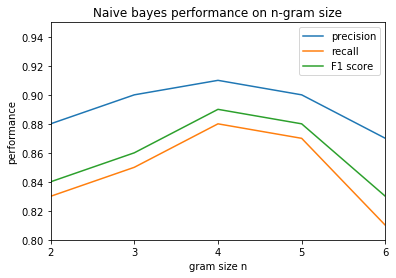
\includegraphics[scale=0.6]{naive.png} \\
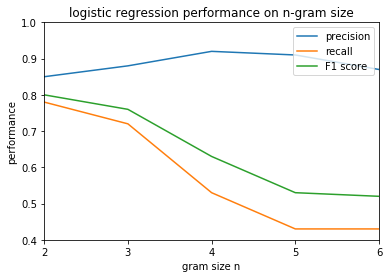
\includegraphics[scale=0.6]{logistic.png} 
%\begin{table}[H]
%\caption {Naive bayes performance on n-gram size}
%\begin{center}
%\begin{tabular}{|c|c|c|c|c|c|}
%\hline 
%size n & 2 & 3 & 4 & 5 & 6 \\ 
%\hline 
%precision & 0.88 & 0.90 & 0.91 & 0.90 & 0.87 \\ 
%\hline 
%recall & 0.83 & 0.85 & 0.88 & 0.87 & 0.81 \\ 
%\hline 
%F1 score & 0.84 & 0.86 & 0.89 & 0.88 & 0.83 \\ 
%\hline 
%\end{tabular} 
%\end{center}
%\end{table}

%\begin{table}[H]
%\caption {Logistic performance on n-gram size}
%\begin{center}
%\begin{tabular}{|c|c|c|c|c|c|}
%\hline 
%size n & 2 & 3 & 4 & 5 & 6 \\ 
%\hline 
%precision & 0.85 & 0.88 & 0.92 & 0.91 & 0.87 \\ 
%\hline 
%recall & 0.78 & 0.72 & 0.53 & 0.43 & 0.43 \\ 
%\hline 
%F1 score & 0.80 & 0.76 & 0.63 & 0.53 & 0.52 \\ 
%\hline 
%\end{tabular} 
%\end{center}
%\end{table}
So based on the two figure above, the best results come from 4-gram.




\section{Multilabel Short Text Language Detection}

There is a growing awareness that over the past two decades, globalization has altered the face of social, cultural and linguistic diversity in societies all over the world. One of the most interesting phenomenon in linguistic is that people tends to mix-use different kind of languages in their daily conversation. One reason is that sometimes the terminology might be easier to understand in one kind of language but not in another one. Or sometimes people try to quote something from other languages, so they just mix-use different kind of languages for convenience. The linguist has showed that when human being try to organize the language, they first form a concept in their imagination and then try to translate this concept into words. Because of the different education background and living environment, there might be some potential problems that can occur when people try to finish the translation:

\begin{itemize}
\item The concept cannot he described in any language.
\item The concept can be described in language A, but language A is not the language that we currently use for the conversation.
\item The concept can be described in language A, and language A is the language that we currently use for the conversation.
\end{itemize}

In the first case there will not be a conversation exist in neither text form or oral form. In the third case, to detect the language is equal to the single-label language detection case, which we already discussed in previous section. The mix-use different kind of language phenomenon happens in the second case. The second phenomenon happens in different register: it is not only happens in oral conversation, but also in some informal written text, for example, text message on Twitter or Facebook. It is a very challenging task to try to detect different kind of languages in short text. In this paper, we call this task \textbf{M}ulti-\textbf{L}abel Language \textbf{D}etection for \textbf{S}hort \textbf{T}ext (MLDST).

MLDST is a challenge task because of two aspects.First, most of the text in MLDST is short, which means we can only extract very limit features from the text itself. Second, in MLDST we are not only try to detect the kind of languages, but we are also try to find the language switch point. Here is a toy example, given the text
\begin{center}
Hello World Hallo Wereld
\end{center}
It is not very helpful if the model only tells us that this text contains English and Dutch. In another way, it would be very helpful if the model can tell us that the first two words are in English and the last two are in Dutch. 

In this section, we try to build a MLDST model using Naive Bayesian and then discuss the possibility of improvement.



\subsection{Data Set}
As in previous section, in this part, we use Bible and Declaration of Human Rights to train the classifier based on Naive Bayesian model. The data set contains 7 languages: Arabic(ar), French(fr), English(en), Russian(ru), Portuguese(pt), Spanish(es) and Indonesia(id).
We use the mixed Twitter data set as the testing data. Later we will give more details about how we create the mixed data set.

Since the data in Twitter data set are all single-label text, i.e. there is only one kind of language in one text sample. We try to create the multi-label data set by ourselves. For simplicity, in this paper, we only consider the case where the text contains two languages: English and Russian. We first randomly select 100 English Twitters and 100 Russian Twitters from our Twitter data set. Then we mix them randomly to get our bi-language Twitter data set. Below is a sample from the mixed data set:

\emph{@ChrisDanielShow between facebook being down this morning and the att cable being cut, its been a hard day for fresno hipsters. @egosh\_69 B 6 yTpa?ecTb?axaxaxa}

In our paper, we only test our model in bi-language Twitter data set. The general idea for multiple-language Twitter data set is the same. 


\subsection{Experiment}
In our MLDST model we try to find the switch between different languages by use the $\log$ probability in Naive Bayesian classifier. More specifically, we try to capture the oscillation of the $\log$ probability in each sub-sentence. 

For each of the mixed Twitter data, we first remove all the noise information like \#, @ emoji, etc. Then we rewrite the text into n-gram format:
\begin{center}
I\_nee \_need need\_ eed\_a ed\_a\_ d\_a\_d \_a\_da a\_day...
\end{center}
Then, in order to observe the Bayesian probability for each sub-sentence, we further change the data into the form in Figure \ref{subsentence}.
\begin{figure}
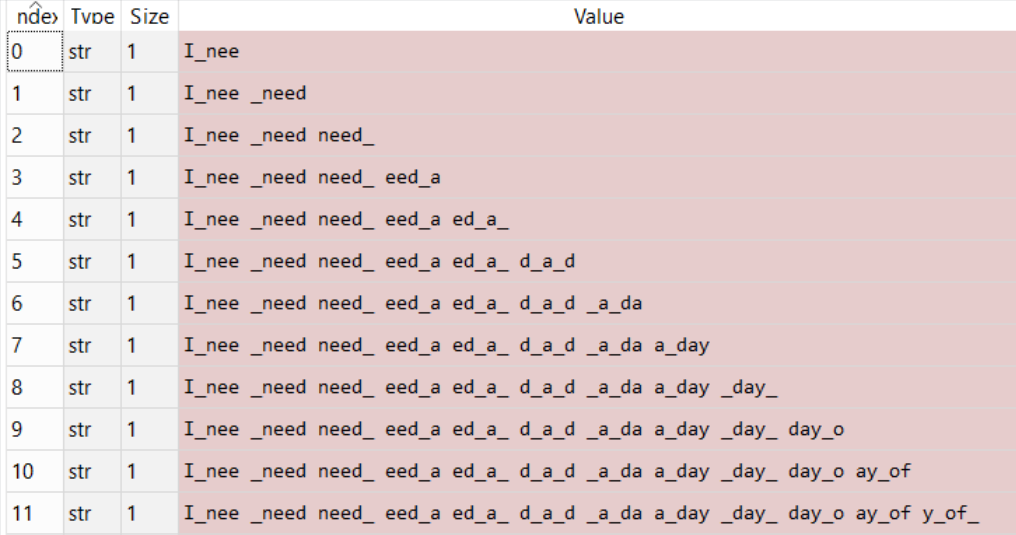
\includegraphics[width=0.5\textwidth]{subsentence.PNG}
\caption{Divide the sentence into some small sub-sentences. In this Figure, we only show the first 12 sub-sentences.}
\label{subsentence}
\end{figure}
For each of the sub-sentence, we feed them into the Naive Bayesian classifier to calculate their log probability belong to each class. We then determine the switch point between different languages by capturing the oscillation in the log probability. 

To make it more clear, let us assume that in the text, the kind of language switch from language A to language B at the $k^{th}$ word. Then it is a reasonable assumption that at the switch point, the log probability of language A becomes decreasing and the log probability of language B becomes increasing, while the log probability of all the other languages should either stay at the same level as before or decreasing. Using above assumption, we try to find the switch by using the log probability for each languages.

To test whether our assumption is true, we created 100 mix-test samples using the English and Russian Twitters. We call it a good prediction if the predicted switch is the same with the true switch. 

\subsection{Results and Analysis}
Below are some plots create using the log probabilities of different languages for different length of sub-sentence. Keep in mind that our mixed Twitter is English+Russian.

As it can be seen in Figure \ref{multilabel_1}, the act of the log probability of different languages for different length of sub-sentence is just about the same with what we predicted in previous section. At the very beginning, the line corresponding to en is the highest one, this indicates that the first half part is in English, which is true. When the index reach 107, the log probability of ru start to increase while the log probability of en is decreasing at that point. So our classifier will predict the switch is at 107, which is correct. 


\begin{figure}
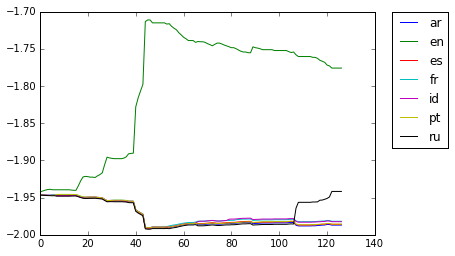
\includegraphics[width=0.5\textwidth]{multilabel_1.PNG}
\caption{The switch point can be detected very well in this example. Since the line represent ru is the only one that increasing at the switch point (which is around 107 in this case).}
\label{multilabel_1}
\end{figure}

In the first example, our classifier predicted the switch correctly. However, our model may fails in some other case. For example, in Figure \ref{multilabel_2}, the switch point cannot be detected very well. in this example the classifier tends to think that the mixed Twitter contains English and French but not English and Russian. This is because at the 13th word, the log probability of French is increasing while the log probability of English is decreasing. We this may because the similarity between English and French is very high, especially under the n-gram setting. Basically, the n-gram only consider the possibility of different combination of alphabets. This will not works very well if the two languages share the same alphabets. 



\begin{figure}
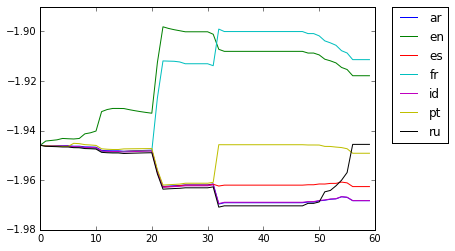
\includegraphics[width=0.5\textwidth]{multilabel_2.PNG}
\caption{The switch point cannot be detected very well in this example. The classifier tends to think that the mixed Twitter contains English and French but not English and Russian. This is because at the 13th word, the log probability of French is increasing while the log probability of English is decreasing. We this may because the similarity between English and French is very high, especially under the n-gram setting.}
\label{multilabel_2}
\end{figure}


In Figure \ref{multilabel_3}, the ru log probability becomes the highest one at the very end, which is good. However, French again becomes the troubler: at 13, the log probability of fr start to increase while the log probability of en decrease. This can fool the classifier and make it think 13 is the switch point but not 26 (which is true switch point).



\begin{figure}
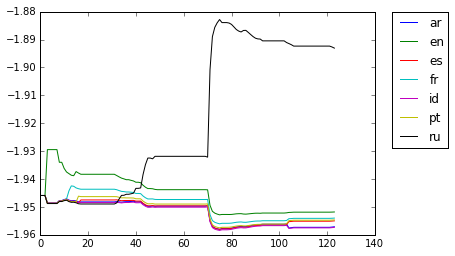
\includegraphics[width=0.5\textwidth]{multilabel_3.PNG}
\caption{There may also be some trouble in this example. Though Russian becomes the one has largest }
\label{multilabel_3}
\end{figure}


The accuracy of final results is not very impressive, amoung 100 mixed test samples, only 23 of the switch are predicted correctly. We think it might because several reasons:
\begin{itemize}
\item The way we extract features(n-gram) can be improved. In this section, due to the limit of time, we only choose one value for n, i.e. n = 5. We think the accuracy can have some mirror improve by choosing different n. Also we think beside to try to set the number of n to be different numbers, we can also try to using other methods to extract features. For example, continuous bag of words can be a potential good method to extract features. 
\item Naive Bayes may not be the best model for this task. Though it is the most intuitive one. 
\item Twitter contains too many noises. Some abbreviation can easily kill the classifier.
\item We think the accuracy can be improved by using some more oral language data set to train to model.
\item The condition to make classification need to be modified or enriched in order to increase the accuracy. For example, besides the increasing and decreasing of the log probability, one may also measure how long the increasing or decreasing last, this can help the classifier to tell the difference between real change and noisy perturbation.
\end{itemize}




\section{Future work and possible improvements}
For single-language short text detection,
the first problem of the method we used here is about the training dataset size, since it's a huge work to extract all chapters from bible, we only extract several chapters for each language, the performance increased from 80\% to 90\% significantly after we increase the number of chapters used form 5 to 20, so if we use more chapters, which means more complete training data, the better performance can be expected.\\
Another issue is that the training data a strictly written language, but the testing data are very informal spoken language, so another possible way to improve the accuracy is to use more informal spoken language text as the training data, but this is another heavy work, which means we need to collect so many different spoken language, we cannot finish this in such a short time.\\
Lastly, we tried recurrent neural network actually, the performance on the testing data is even below 80\%, which means it's below the simple frequency accuracy, if we more time, we should be able to figure out the problem and improve the performance.

For multi-language short text detection, we think the future work may contains below aspects:
\begin{itemize}
\item Different feature extraction method.
\item Try more oral language training data set.
\item Try some models other than Naive Bayes. 
\end{itemize}
To the best of our knowledge, this paper is the first one try to conquer the multi-label short text language detection problem. We are not only try to find the number of different languages, but also try to detect the switch point, which makes this problem very challenge. Though the result is not very impressive, but it can be a baseline of this kind of problems and also our experience can be helpful for other researchers who interested in this problem.


\section{Acknowledgments}
We would like to thank Dr. Chai for her excellent teaching during the fall semester and inspiring us on this problem.


\begin{thebibliography}{}

\bibitem[\protect\citename{Aho and Ullman}1972]{Aho:72}
Jan Blommaert and Ben Rampton.
\newblock 1972.
\newblock {\em Language and Superdiversity}.
\newblock Diversities Vol. 13, No. 2, 2011, ISSN 2079-6595, www.unesco.org/shs/diversities/vol13/issue2/art1 © UNES CO.
\

\end{thebibliography}



\end{document}